\subsection{Repository-Service-Controller}

\begin{figure}[H] 
    \centering 
    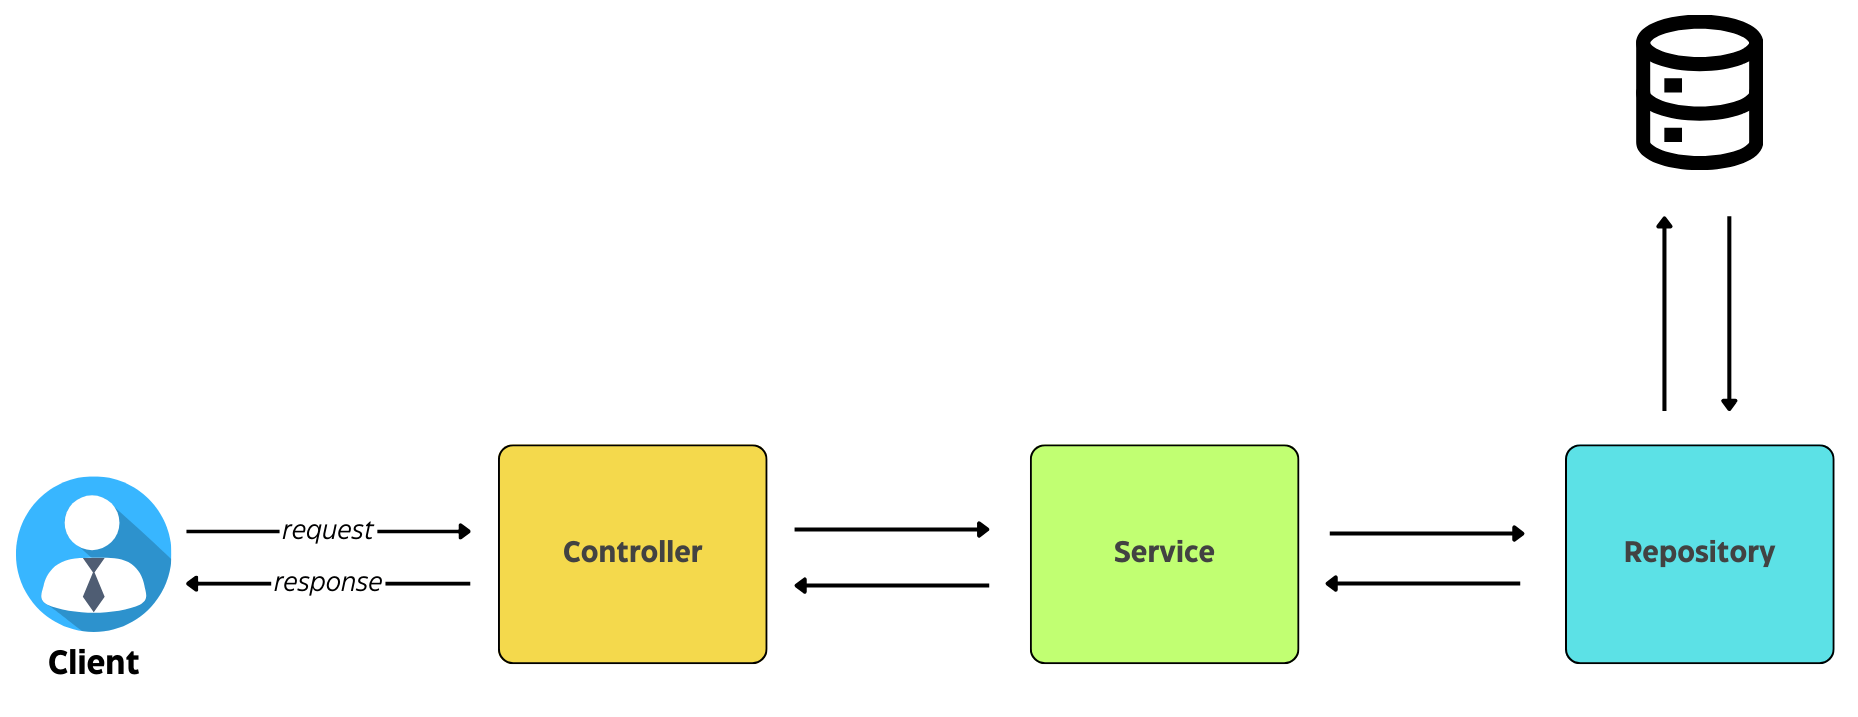
\includegraphics[width=0.90\columnwidth]{rep-serv-contr-custom} 
    \caption{Schema di collegamento tra i componenti Controller, Service e Repository}
\end{figure}

\noindent In un'applicazione Spring Boot che implementa una REST API l'interazione tra questi tre componenti è fondamentale per gestire le richieste HTTP, elaborare la business logic e interagire con il database.\\
Come descritto nell'immagine l'interazione tra i componenti segue questo flusso:
\begin{enumerate}
\item il client invia una richiesta HTTP e arriva al Controller tramite URL;
\item il controller estrae i dati della richiesta, effettua controlli di validazione e chiama il metodo del service appropriato;
\item il metodo del service invocato conterrà la business logic per eseguire la richiesta e ulteriori controlli di validazione;
\item la/le repository coinvolta/e ottengono i dati richiesti dal database che vengono restituiti al service che li rielaborerà, restituitendo il risultato al controller;
\item il controller crea una risposta appropriata in formato JSON e la restituisce al client.
\end{enumerate}

\subsubsection{Controller}
\begin{figure}[H] 
    \centering 
    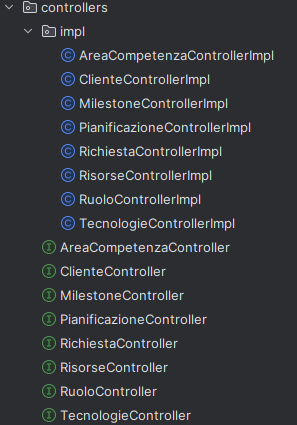
\includegraphics[width=0.4\columnwidth]{controllers} 
    \caption{Controller sviluppati}
\end{figure}
Il Controller è punto di instradamento per le richieste HTTP. Riceve le richieste dal client, estrae i dati dai parametri della richiesta o dal corpo (body), esegue appropriati controlli di validazione ed infine inoltra le operazioni al Service. I controlli di validazione comprendono: validazione degli UUID, validazione del formato delle date inserite, validazione che un dato obbligatorio non sia nullo e controllo che i filtri inseriti non siano non valorizzati.\\
Ogni Controller è formato dalla sua interfaccia, contenente la firma dei metodi associati agli endpoint, e dalla sua implementazione. Ognuno di essi è annotato con \textit{@RestController}.

\begin{figure}[H] 
    \centering 
    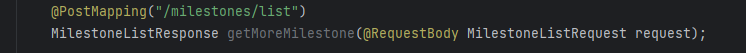
\includegraphics[width=0.9\columnwidth]{controller-interfaccia} 
    \caption{Firma di un metodo nell'interfaccia di un Controller}
\end{figure}
\noindent All'interno dell'interfaccia del Controller troviamo tutti i metodi associati agli endpoint. Per identificare a quale endpoint appartiene vengono utilizzate annotazioni come: \textit{@PostMapping}, \textit{@GetMapping}, \textit{@DeleteMapping}, \textit{@PutMapping} e \textit{@PatchMapping}.\\
Tramite l'annotazione \textit{@RequestBody} Spring deserializza\textsubscript{g} automaticamente il JSON in un tipo Java, in questo caso \texttt{MilestoneListRequest}.
Come libreria standard utilizzata per mappare i campi JSON inseriti nella request dall'utente in un oggetto Java è la libreria Jackson\textsubscript{g}.

\begin{figure}[H] 
    \centering 
    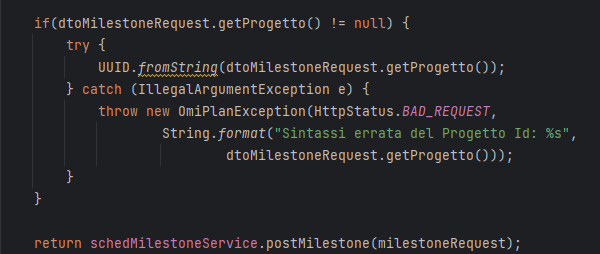
\includegraphics[width=0.8\columnwidth]{controller-validazione} 
    \caption{Esempio di controllo di validazione}
\end{figure}
\noindent Nelle classi \texttt{ControllerImpl} troviamo l'implementazione dei metodi dell'interfaccia, controlli di validazione che possono lanciare eccezioni e il metodo del Service utilizzato.\\
In questo code snippet vediamo il controllo di validazione su l'Id del Progetto associato ad una Milestone. Se passerà il controllo, allora verrà inoltrata la richiesta al Service.

\subsubsection{Repository}
\begin{figure}[H] 
    \centering 
    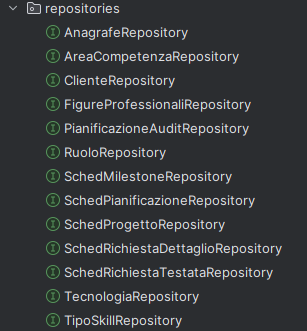
\includegraphics[width=0.4\columnwidth]{repositories} 
    \caption{Repository sviluppati}
\end{figure}
Un Repository in Spring Boot fornisce un modo per interagire con una fonte di dati, in questo caso un database. Permette di eseguire operazioni CRUD tramite Spring Data JPA che genera automaticamente query SQL in base ai metodi che l'interfaccia del Repository contiene.\\
Le Repository da me create estendono, per poter eseguire le query, estendono l'interfaccia \texttt{JpaRepository} o \texttt{ PagingAndSortingRepository} per risposte paginate.\\
Ogni Repository deve essere annotato con \textit{@Repository}. 
\begin{figure}[H] 
    \centering 
    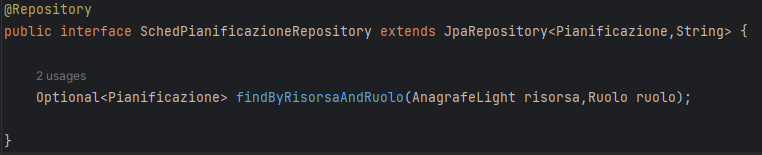
\includegraphics[width=0.9\columnwidth]{repository-example} 
    \caption{Esempio di una Repository}
\end{figure}
\noindent È possibile creare delle query personalizzate SQL tramite parole chiave di Spring Data JPA. In questo caso nell'immagine la query corrisponderà alla ricerca della Pianificazione che ha la stessa Risorsa e lo stesso Ruolo.

\subsubsection{Service}
\begin{figure}[H] 
    \centering 
    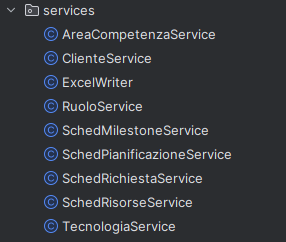
\includegraphics[width=0.4\columnwidth]{services} 
    \caption{Service sviluppati}
\end{figure}
Il Service è un componente che contiene elaborazioni di dati, chiamate a metodi nei Repository per accedere al database e restituisce i risultati al Controller.\\
Ogni Service è annotato con annotato \textit{@Service}.\\
\begin{figure}[H] 
    \centering 
    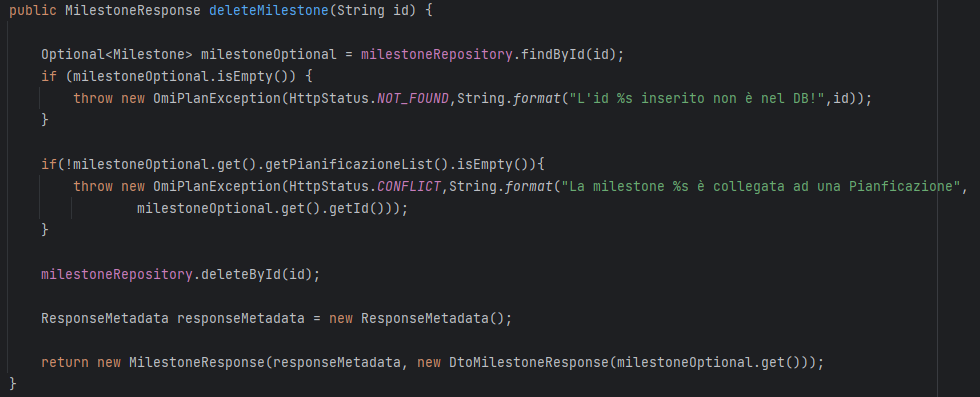
\includegraphics[width=0.95\columnwidth]{service-delete-example} 
    \caption{Metodo deleteMilestone() nel Service}
\end{figure}
\noindent In questo code snippet possiamo osservare come funziona il metodo \texttt{deleteMilestone()} all'interno del \texttt{MilestoneService}. Viene controllato, tramite un metodo fornito dal repository della Milestone se l'ID è presente nel database e in caso positivo viene sollevata un'eccezione che interrompe la cancellazione della Milestone. Il controllo successivo verifica che la Milestone non sia collegata ad una Pianificazione ed in caso di esito positivo interrompere la cancellazione.\\
Se tutti questi controlli risultano negativi allora avverrà la cancellazione nel database, tramite il metodo fornito dal repository della Milestone, della Milestone associata a quell'ID. Viene infine generata la response da ritornare al Controller formata da un oggetto metadata vuoto, dato che non ci sono stati errori, e una nuova \texttt{MilestoneResponse}.\\\\
Un altro metodo rilevante utilizzato nei Service è quello utilizzato per la generazione della query personalizzata in base ai filtri inseriti dall'utente.\\
Dato che la query con Spring Data JPA sarebbe stata troppo lunga e poco leggibile, è stato deciso di crearla tramite \textit{CriteriaBuilder}\textsubscript{g} e \textit{CriteriaQuery}\textsubscript{g} che permettono di creare query dinamiche in modo programmatico.
\begin{figure}[H] 
    \centering 
    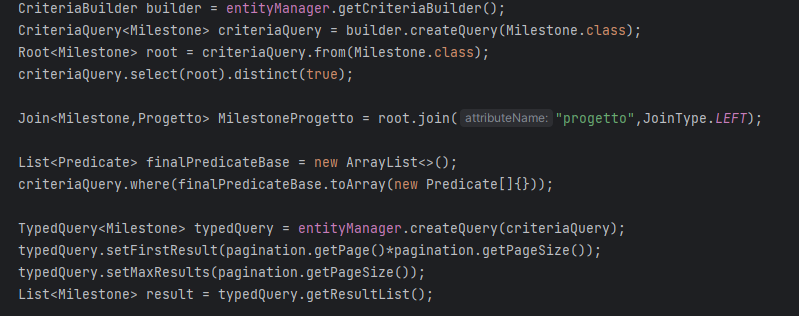
\includegraphics[width=0.95\columnwidth]{criteriaquery} 
    \caption{Code snippet della creazione della query basata su filtri inseriti}
\end{figure}
\noindent In questo frammento di codice, ho semplificato la creazione della query dinamica, lasciando i punti chiave che spiegano il funzionamento.\\
Nel primo blocco di istruzioni inizializziamo CriteriaBuilder, una nuova CriteriaQuery e selezioniamo tutti i campi dell'entità \texttt{Milestone}.\\
Nelle successive istruzioni andiamo a creare tutte le operazioni di \textit{Join<>} tra le entità, inseriamo dei predicati (condizioni logiche, utili quando la query è dinamica) nella clausola \texttt{where()} della query e infine generiamo la query simulando la paginazione recuperando la lista di risultati in una Lista di \texttt{Milestone}.


\subsection{Swagger UI}
Spiegazione come è stata creata la grafica per gli endpoint con screen di un'interfaccia Controller.